% !TEX root = ../my-thesis.tex
%

\chapter{Introducción}
\label{sec:intro}

\cleanchapterquote{You can’t do better design with a computer, but you can speed up your work enormously.}{Wim Crouwel}{(Graphic designer and typographer)}


En el presente capitulo se expone el objetivo general, así como sus derivados. En la
primera sección se aborda el tema de investigación donde especifica la justificación del
presente trabajo, posteriormente se sintetiza algunas de las investigaciones que sirvieron
como base para la elección del tema previamente descrito. Finalmente se dan las razones
de la investigación y se exponen las aportaciones derivadas del tema de tesis.

\section{Tema de investigación}
En el campo de la aeronáutica hay una rama que en los últimos años ha sido objeto
de estudio debido a su exponencial importancia para tareas criticas, se trata de los
vehículos aéreos no tripulados UAV (del inglés unmanned aerial vehicle), donde dichas
tareas criticas han podido alcanzar sus objetivos en parte gracias a la implementación
reciente de visión artificial.\\
En la implementación de cámaras para el sistema visual de los UAV's la estabilidad
juega un rol importante, debido a que el sistema se encuentra expuesto a diversos
factores que hacen que la captura de imágenes sea deficiente. Es por ello que la
implementación de un sistema estabilizador de cámaras en necesario.\\
Tareas tales como la geo-localizacion requieren como entrada ángulos de azimuth
y de elevación que son entregadas por el sistema gimbal embebido en el UAV.
El algoritmo de geo-localización utiliza la salida del GPS, el vector de línea de
visión normalizado del algoritmo de visión y la actitud para estimar la posición del
objeto en el marco de inercia y la distancia al objeto.

\section{Justificación}
La presente investigación se enfocara en la implementación de una gimbal de dos grados
de libertad utilizando un framework de código abierto y bajo la licencia de Open-Source
siendo este el motivo principal de contribuir a la comunidad y el de la creación de
un repositorio de libre acceso para futuras investigaciones y mejoramiento de la calidad.\\
Para la universidad aeronáutica en Querétaro representara solo el inicio de una potencial
investigación en MAV'S \footnote{Micro air vehicle}.

\section{Objetivo}
%%%%%%%%%%%%%%%%%%%%%%%%%%%%%%%%%%%%%%%%%%%%%%%%%%%%%%%%%%%%%%%%%%%%%%%%%
%Se escribe en infinitivo y resuelve las preguntas ¿Que? ¡Como? y ¿para que? %
%%%%%%%%%%%%%%%%%%%%%%%%%%%%%%%%%%%%%%%%%%%%%%%%%%%%%%%%%%%%%%%%%%%%%%%%%
Diseñar, instrumentar y controlar un dispositivo gimbal que sea capaz de seguir un objeto a través de visión artificial para
implementarse en un UAV de categoría pequeña a velocidad baja.
\begin{figure}[htb]
	\centering
	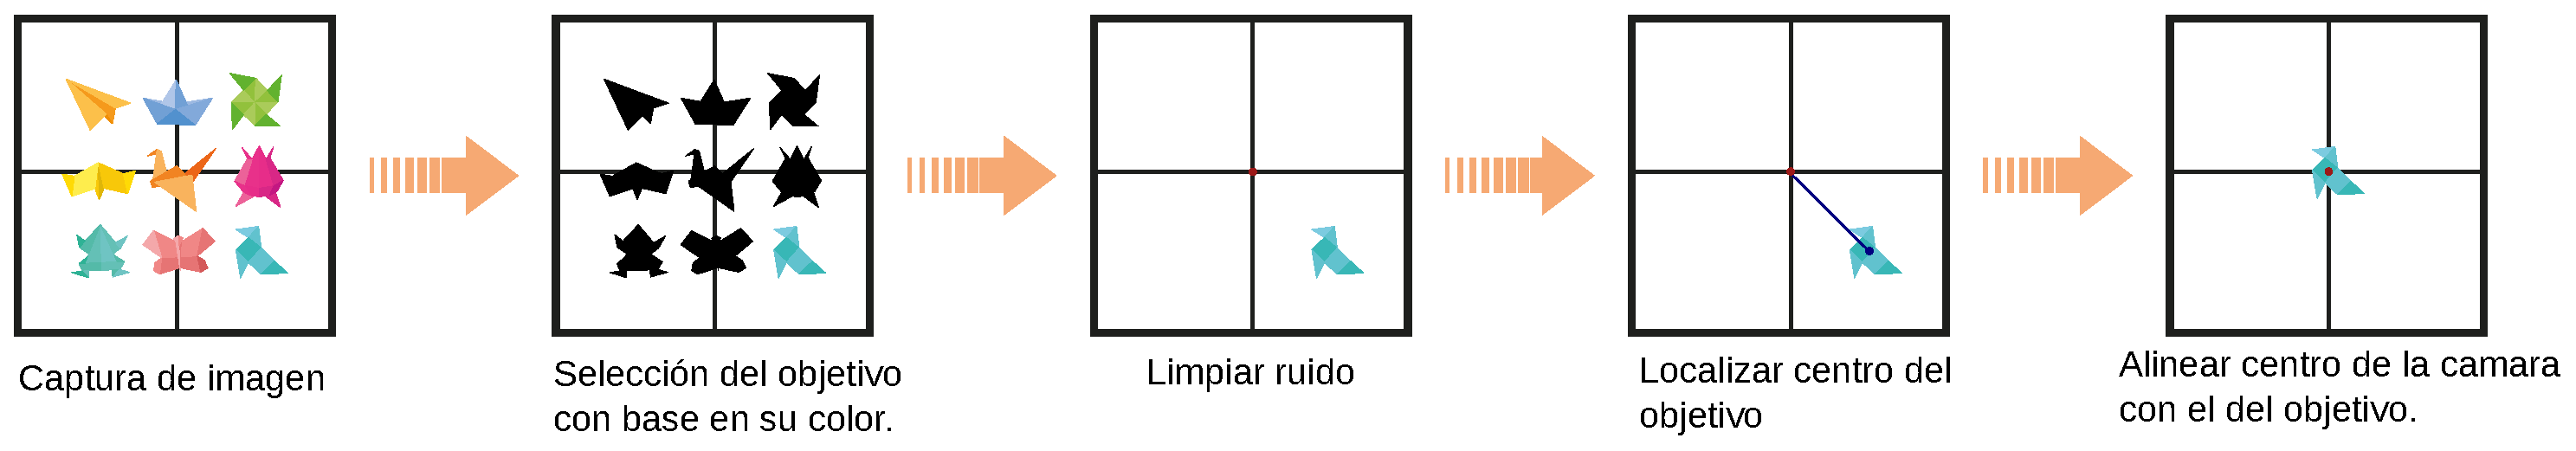
\includegraphics[width=0.85\textwidth]{Contenido/Cuerpo/Capitulo1/Fig0.eps}
	\captionof{figure}{Representación grafica del objetivo del proyecto}
	\label{fig:Introduccion:Fig1}
\end{figure}

\section{Objetivos específicos}
%%%%%%%%%%%%%%%%%%%%%%%%%%%%%%%%%%%%%%%%%%%%%%%%%%%%%%%%%%%%%%%%%%%%%%%%%
%Seran los capitulos de la tesis %
%%%%%%%%%%%%%%%%%%%%%%%%%%%%%%%%%%%%%%%%%%%%%%%%%%%%%%%%%%%%%%%%%%%%%%%%%
\begin{itemize}
	\item Obtener el modelo matemático de una gimbal.
	\item Diseñar e implementar el sistema embebido que dará el soporte electrónico a la gimbal.
	\item Capturar figuras geométricas definidas  mediante el uso de una cámara digital y emplear algoritmos de visión artificial para la obtención de datos.
	\item Diseñar un controlador autónomo con base en el modelo matemático, previamente obtenido.
\end{itemize}

\section{Estado de la cuestion}
%%%%%%%%%%%%%%%%%%%%%%%%%%%%%%%%%%%%%%%%%%%%%%%%%%%%%%%%%%%%%%%%%%%%%%%%%
%Descripción breve de las obras, proyectos, intentos universitarios más significativos %
%%%%%%%%%%%%%%%%%%%%%%%%%%%%%%%%%%%%%%%%%%%%%%%%%%%%%%%%%%%%%%%%%%%%%%%%%
La aparición de la gimbal no es un termino para nada nuevo, de hecho es viejo más de lo que
muchos podemos creer. Fue en el 250 antes de nuestra era cuando el inventor Philo of Byzantium
describió un bote de tinta de ocho lados con una abertura en cada lado, que se puede
girar de modo que mientras cualquier cara está en la parte superior, se puede sumergir y
entintar un bolígrafo, aunque la tinta nunca se agota a través de los agujeros de los otros
lados. \cite{WEB:Gimbal}\\
Desde entonces y hasta la fecha múltiples científicos han desarrollado investigaciones alrededor
de dicho artefacto, algunos teniendo más éxito que otros; los cuales serán brevemente expuestos
con la finalidad de obtener el estado actual en el que se encuentra la gimbal y su avance
tecnológico.
\begin{itemize}
	\item \textbf{Navegación inercial}\\
	      En la navegación inercial, como se aplica a los barcos y submarinos, se necesita
	      un mínimo de tres gimbals para permitir que un sistema de navegación inercial
	      (masa estable) permanezca fijo en el espacio inercial, compensando los cambios
	      en el guiñada, inclinación y balanceo del barco.
	      \begin{figure}[htb]
		      \centering
		      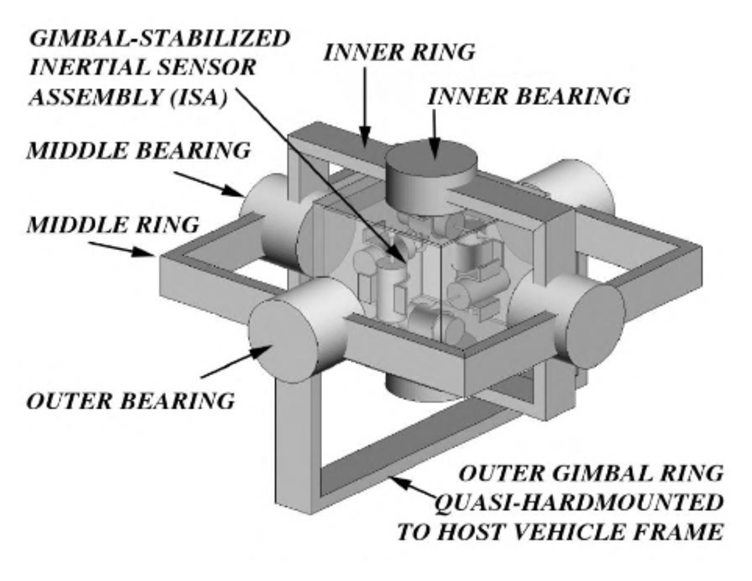
\includegraphics[width=0.6\textwidth]{Contenido/Cuerpo/Capitulo1/Fig1.eps}
		      \captionof{figure}{Uso de una gimbal para un sensor inercial \cite{Book:InNav}}
		      \label{fig:Introduccion:Fig2}
	      \end{figure}

	      En esta aplicación, la Unidad de medición inercial (IMU) está equipada con tres
	      giroscopios montados ortogonalmente para detectar la rotación alrededor de todos
	      los ejes en el espacio tridimensional. Las salidas giroscópicas accionan motores
	      que controlan la orientación de los tres gimbal según sea necesario para mantener
	      la orientación de la IMU.

	\item \textbf{Motores de cohete}\\
	      En la propulsión de naves espaciales, los motores de cohetes generalmente se
	      montan en un par de gimbals para permitir que un solo motor logre el empuje
	      sobre los ejes de inclinación y guiñada; o, a veces, solo se proporciona un eje
	      por motor. Para controlar el giro, se utilizan motores gemelos con señales de
	      control de inclinación diferencial o guiñada para proporcionar torque sobre el
	      eje de balanceo del vehículo.\\
	      Uno de los motores más famosos es el J-2X.Es un motor de cohete avanzado altamente
	      eficiente y versátil con las características ideales de empuje y rendimiento para
	      impulsar la etapa superior del espacio de la NASA.\cite{WEB:NASA}
	      \begin{center}
		      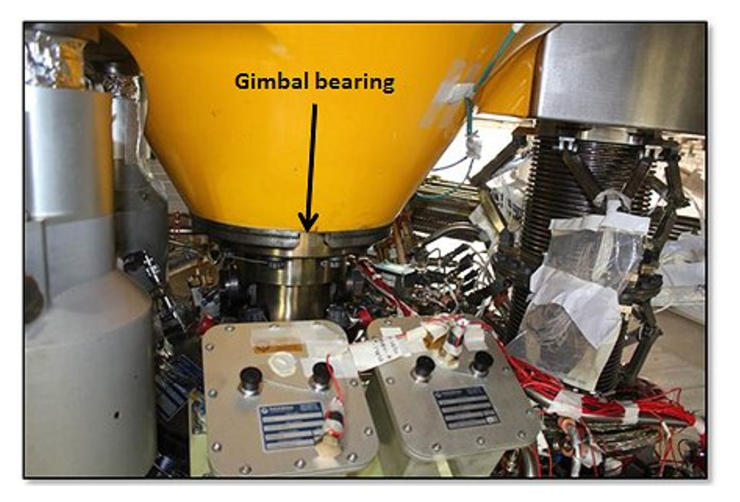
\includegraphics[width=0.4\textwidth]{Contenido/Cuerpo/Capitulo1/Fig2.eps}
		      \captionof{figure}{Uso de una gimbal en un motor de propulsión \cite{WEB:NASA2JX} }
		      \label{fig:Introduccion:Fig3}
	      \end{center}

	\item \textbf{Entrenamiento para astronautas}\\
	      Sistema de simulación de maniobras de tipo caída que se pueden encontrar en el vuelo espacial
	      fue creado por la NASA y era conocido como "the gimbal rig,".
	      Tres jaulas tubulares de aluminio podrían girar por separado o en combinación para
	      dar movimientos de balanceo, cabeceo y guiñada a velocidades de hasta 30
	      revoluciones por minuto, mayores que las esperadas en vuelos espaciales reales.
	      Los chorros de gas nitrógeno, unidos a las tres jaulas, controlaron el movimiento.
	      Desde el 15 de febrero hasta el 4 de marzo de 1960, la plataforma de cardán
	      proporcionó una capacitación valiosa para los siete astronautas del Proyecto
	      Mercurio. Cada uno experimentó unas cinco horas de tiempo de vuelo simulado.\cite{WEB:MERCURY}
	      \begin{center}
		      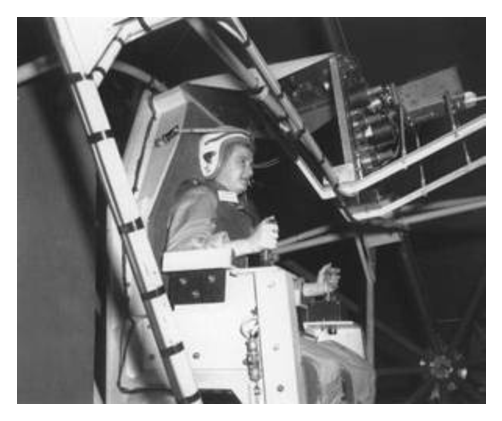
\includegraphics[width=0.6\textwidth]{Contenido/Cuerpo/Capitulo1/Fig3.eps}
		      \captionof{figure}{Jerrie Cobb, uno de los Mercury 13, da un giro en la plataforma gimbal.
			      Créditos: NASA }
		      \label{fig:Introduccion:Fig4}
	      \end{center}

	\item \textbf{Estabilizador de Camaras}\\
	      Los gimbals también se utilizan para montar todo, desde lentes de cámara pequeñas
	      hasta telescopios fotográficos grandes.\\
	      En los equipos de fotografía portátiles, se utilizan gimbals de un
	      solo eje para permitir un movimiento equilibrado de la cámara y las lentes.
	      Esto resulta útil en la fotografía semi-profesional, así como en cualquier otro
	      caso en el que se adopten teleobjetivos muy largos y pesados: un eje de la gimbal
	      gira un lente alrededor de su centro de gravedad, lo que permite una manipulación
	      fácil y suave mientras se rastrea a los sujetos en movimiento.\\
	      Los montajes de gimbal muy grandes en forma de montajes de altitud-altitud de 2 o 3 ejes
	      se utilizan en la fotografía satelital con fines de seguimiento.\\
	      En la década de 1970, el director de fotografía estadounidense Garrett Brown tuvo
	      una idea simple pero revolucionaria: hacer un dispositivo que pudiera suavizar las
	      tomas de acción manuales.
	      \begin{center}
		      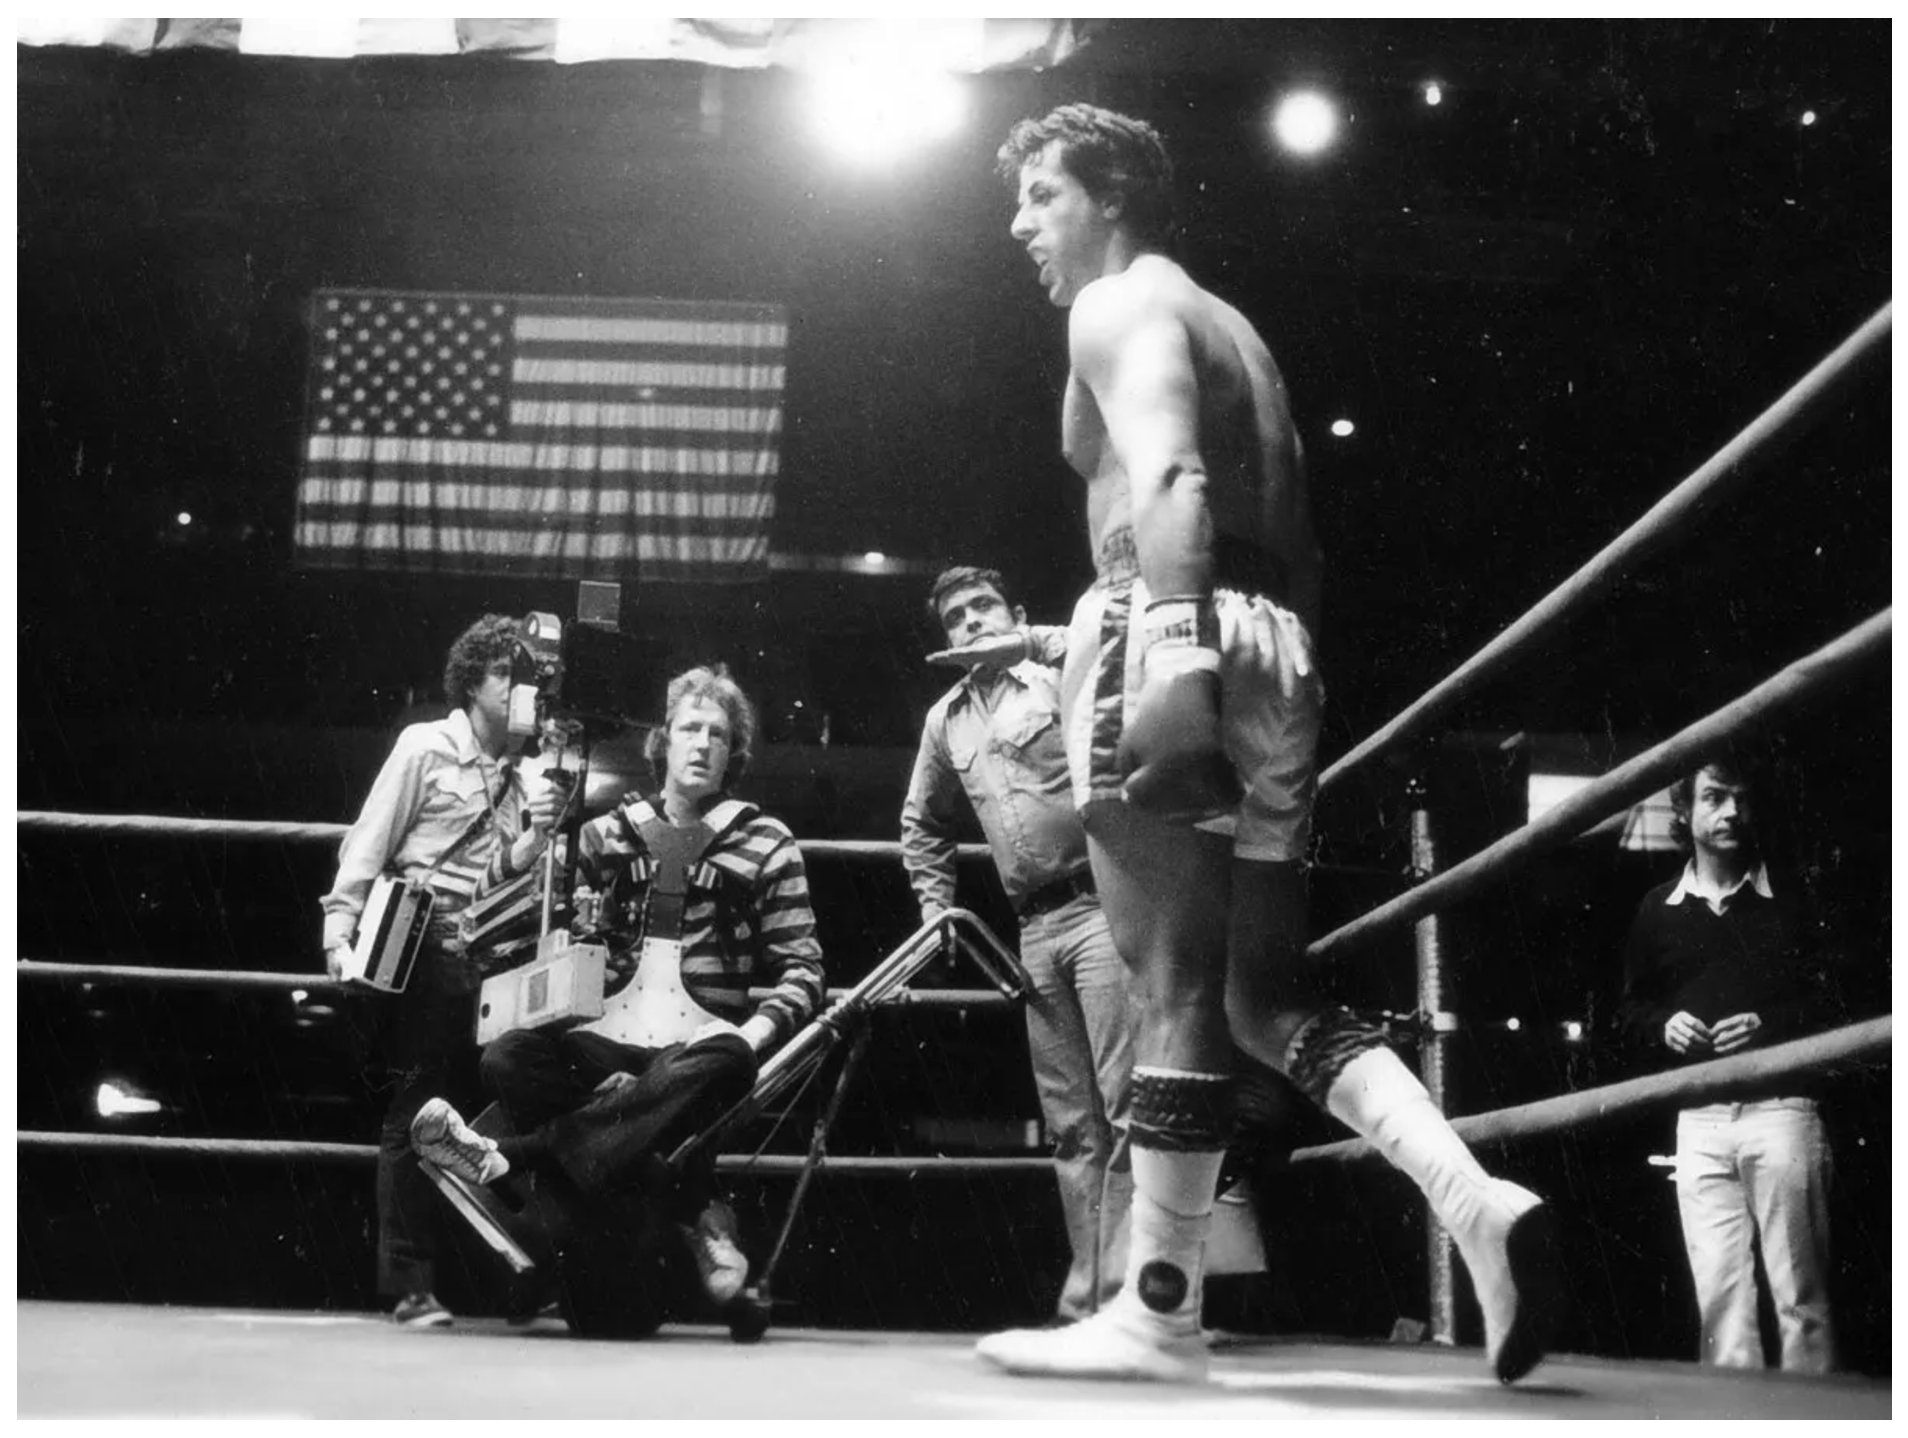
\includegraphics[width=0.5\textwidth]{Contenido/Cuerpo/Capitulo1/Fig4.eps}
		      \captionof{figure}{Primer uso de la steadicam}
		      \label{fig:Introduccion:Fig5}
	      \end{center}

	      El resultado es el Steadicam (Que cumple con los principios físicos de la gimbal).
	      Ganador de un Premio de la Academia, que hizo su debut cinematográfico en la
	      película "Bound for Glory", y se destacó en las películas "Rocky" y "The Shining"


\end{itemize}

\section{Contribuciones}
%%%%%%%%%%%%%%%%%%%%%%%%%%%%%%%%%%%%%%%%%%%%%%%%%%%%%%%%%%%%%%%%%%%%%%%%%
%                         Contribuciones                                %
%%%%%%%%%%%%%%%%%%%%%%%%%%%%%%%%%%%%%%%%%%%%%%%%%%%%%%%%%%%%%%%%%%%%%%%%%
Actualmente la forma en que se desarrollan los sistemas gimbal de los vehículos aéreos no tripulados están basados en el procesamiento
de datos con Arduino conectado a ROS, la idea de migrar a una tarjeta micro controladora mas fiable como la TMS570LC43 hace que esta sea una
de las principales aportaciones, ya que queda bajo licencia de software libre, además de la investigación en mejorar el algoritmo de búsqueda
de centroide de la visión artificial, mediante el uso de corrección de factor gamma. Lo que nos puede permitir ajustar los filtros con un sensor 
de luminancia\\
A nivel escolar, es la primera tesis que incluye visión artificial en la carrera de Ingeniería Electrónica y Control de Sistemas de Aeronaves, 
siendo esta investigación el inicio de un proyecto de instrumentación de MAV con la incorporación de una tarjeta monoprocesador con ROS.

\section{Alcances}
%%%%%%%%%%%%%%%%%%%%%%%%%%%%%%%%%%%%%%%%%%%%%%%%%%%%%%%%%%%%%%%%%%%%%%%%%
%¿Porque es relevante la solucion o mejora o implementacion.? ¿por que es novedosa? %
%%%%%%%%%%%%%%%%%%%%%%%%%%%%%%%%%%%%%%%%%%%%%%%%%%%%%%%%%%%%%%%%%%%%%%%%%
La investigacion actual tiene los siguientes alcances:
\begin{itemize}
	\item Hacer el control para dos grados de libertad.
	\item Utilizar filtros morfologicos(opening y closing).
	\item Que la variacion de gamma sea por software y no por hardware
	\item No sera acoplado a un vehiculo aereo, queda en simulación en tierra.
\end{itemize}


% \section{Estructura de la tesis}